% Options for packages loaded elsewhere
\PassOptionsToPackage{unicode}{hyperref}
\PassOptionsToPackage{hyphens}{url}
\documentclass[
  10pt,
]{article}
\usepackage{xcolor}
\usepackage[margin=2.2cm]{geometry}
\usepackage{amsmath,amssymb}
\setcounter{secnumdepth}{-\maxdimen} % remove section numbering
\usepackage{iftex}
\ifPDFTeX
  \usepackage[T1]{fontenc}
  \usepackage[utf8]{inputenc}
  \usepackage{textcomp} % provide euro and other symbols
\else % if luatex or xetex
  \usepackage{unicode-math} % this also loads fontspec
  \defaultfontfeatures{Scale=MatchLowercase}
  \defaultfontfeatures[\rmfamily]{Ligatures=TeX,Scale=1}
\fi
\usepackage{lmodern}
\ifPDFTeX\else
  % xetex/luatex font selection
\fi
% Use upquote if available, for straight quotes in verbatim environments
\IfFileExists{upquote.sty}{\usepackage{upquote}}{}
\IfFileExists{microtype.sty}{% use microtype if available
  \usepackage[]{microtype}
  \UseMicrotypeSet[protrusion]{basicmath} % disable protrusion for tt fonts
}{}
\makeatletter
\@ifundefined{KOMAClassName}{% if non-KOMA class
  \IfFileExists{parskip.sty}{%
    \usepackage{parskip}
  }{% else
    \setlength{\parindent}{0pt}
    \setlength{\parskip}{6pt plus 2pt minus 1pt}}
}{% if KOMA class
  \KOMAoptions{parskip=half}}
\makeatother
\usepackage{longtable,booktabs,array}
\newcounter{none} % for unnumbered tables
\usepackage{calc} % for calculating minipage widths
% Correct order of tables after \paragraph or \subparagraph
\usepackage{etoolbox}
\makeatletter
\patchcmd\longtable{\par}{\if@noskipsec\mbox{}\fi\par}{}{}
\makeatother
% Allow footnotes in longtable head/foot
\IfFileExists{footnotehyper.sty}{\usepackage{footnotehyper}}{\usepackage{footnote}}
\makesavenoteenv{longtable}
\usepackage{graphicx}
\makeatletter
\newsavebox\pandoc@box
\newcommand*\pandocbounded[1]{% scales image to fit in text height/width
  \sbox\pandoc@box{#1}%
  \Gscale@div\@tempa{\textheight}{\dimexpr\ht\pandoc@box+\dp\pandoc@box\relax}%
  \Gscale@div\@tempb{\linewidth}{\wd\pandoc@box}%
  \ifdim\@tempb\p@<\@tempa\p@\let\@tempa\@tempb\fi% select the smaller of both
  \ifdim\@tempa\p@<\p@\scalebox{\@tempa}{\usebox\pandoc@box}%
  \else\usebox{\pandoc@box}%
  \fi%
}
% Set default figure placement to htbp
\def\fps@figure{htbp}
\makeatother
% definitions for citeproc citations
\NewDocumentCommand\citeproctext{}{}
\NewDocumentCommand\citeproc{mm}{%
  \begingroup\def\citeproctext{#2}\cite{#1}\endgroup}
\makeatletter
 % allow citations to break across lines
 \let\@cite@ofmt\@firstofone
 % avoid brackets around text for \cite:
 \def\@biblabel#1{}
 \def\@cite#1#2{{#1\if@tempswa , #2\fi}}
\makeatother
\newlength{\cslhangindent}
\setlength{\cslhangindent}{1.5em}
\newlength{\csllabelwidth}
\setlength{\csllabelwidth}{3em}
\newenvironment{CSLReferences}[2] % #1 hanging-indent, #2 entry-spacing
 {\begin{list}{}{%
  \setlength{\itemindent}{0pt}
  \setlength{\leftmargin}{0pt}
  \setlength{\parsep}{0pt}
  % turn on hanging indent if param 1 is 1
  \ifodd #1
   \setlength{\leftmargin}{\cslhangindent}
   \setlength{\itemindent}{-1\cslhangindent}
  \fi
  % set entry spacing
  \setlength{\itemsep}{#2\baselineskip}}}
 {\end{list}}
\usepackage{calc}
\newcommand{\CSLBlock}[1]{\hfill\break\parbox[t]{\linewidth}{\strut\ignorespaces#1\strut}}
\newcommand{\CSLLeftMargin}[1]{\parbox[t]{\csllabelwidth}{\strut#1\strut}}
\newcommand{\CSLRightInline}[1]{\parbox[t]{\linewidth - \csllabelwidth}{\strut#1\strut}}
\newcommand{\CSLIndent}[1]{\hspace{\cslhangindent}#1}
\setlength{\emergencystretch}{3em} % prevent overfull lines
\providecommand{\tightlist}{%
  \setlength{\itemsep}{0pt}\setlength{\parskip}{0pt}}
\usepackage{bookmark}
\IfFileExists{xurl.sty}{\usepackage{xurl}}{} % add URL line breaks if available
\urlstyle{same}
\hypersetup{
  pdftitle={OMC at TREC 2026 AutoJudge: Methods and Results},
  pdfauthor={Max Irwin; Nathan Day; Daniel Worley},
  hidelinks,
  pdfcreator={LaTeX via pandoc}}

\title{OMC at TREC 2026 AutoJudge: Methods and Results}
\usepackage{etoolbox}
\makeatletter
\providecommand{\subtitle}[1]{% add subtitle to \maketitle
  \apptocmd{\@title}{\par {\large #1 \par}}{}{}
}
\makeatother
\subtitle{Conference notebook paper}
\author{Max Irwin\footnote{\href{mailto:max@onemorecloud.com}{\nolinkurl{max@onemorecloud.com}}} \and Nathan
Day\footnote{\href{mailto:nday@eezy.com}{\nolinkurl{nday@eezy.com}}} \and Daniel
Worley\footnote{\href{mailto:dworley@gmail.com}{\nolinkurl{dworley@gmail.com}}}}
\date{10 November 2026}

\begin{document}
\maketitle

\subsection{Abstract}\label{abstract}

Decision models offer a novel (and cheaper) alternative to the
established LLM-as-a-judge paradigm
(\citeproc{ref-zheng2023judging}{Zheng et al. 2023}). Jev, the first
decision model publicly released in September 2026, changes the output
of a large pre-trained model from the free-form-text of LLMs to a
type-safe-selection from a pre-defined set of options. Jev also emits a
confidence score for each of its decisions and it offers all of this at
an order of magnitude cheaper inference costs. Our submissions explore
Jev's performance as a both pair-wise-response judge and one-shot-QREL
judge. We also explore a prompt enrichment strategey known as
`bag-of-decisions' leveraging a traditional LLM to build an ``enriched''
request for Jev grading.

\section{1. Introduction}\label{introduction}

LLM-as-a-judge has made relevance assesement cheaper than ever. While
LLM-judges have become more common in industry applications and create
compelling output judgements, they still exhibit major drawbacks that
limit their functional utility including: positional-bias
(\citeproc{ref-wang2024large}{Wang et al. 2024}), self-preference
(\citeproc{ref-panickssery2024llm}{Panickssery et al. 2024}),
score-centrality and over-confidence. Methods to address these short
comings often involed spending more time ``reasoning'', running more
permutation-prompts per single assesment, running several foundations
LLMs in a judge-panel, all of which add to expense and over-confidence
as context is expanded. We explore the utility of a `bag of decisions'
context enrichment step that uses a separate LLM to build a evaluation
rubric of specific yes/no questions that are then used to subsequent Jev
prompt.

Jev is a decision model that takes advantage of similar web-scale
pre-training like an LLM, but instead of generating free-form-text
output, it instead produces an decision based on a prompt-defined
rubric. Unlike LLM-defined-rubrics Jev's training regime makes
hallucination impossible and rubric adherence absolute. Jev supports
making three classes of decision: Noul, Choice and Score. All of which
are accompanied by a confidence score.

We also propose two smaller model strategies to be used alongside larger
models. The first is Hallucination-Risk (HR), which works independent of
LLM or Jev using spaCy (\citeproc{ref-honnibal2017spacy}{Honnibal and
Montani 2017}) noun-phrase detection to build an index of concepts for
each topic that allows foreground/background calculations for a given
run. The second we include is miniLM's
(\citeproc{ref-wang2020minilm}{Wang et al. 2020}) cosine similarity
between a topic and response, which gives us a useful marker for
``easy'' compared to ``hard'' examples.

\section{2. Approach}\label{approach}

Our approaches are aimed at measuring Jev's utility as a judge, at both
levels of RAG relevance assesment. We judge at both the response and the
citation level to compare the quality of the assesment to the cost.
Along the way we explore and try to mitigate Jev's suseptibility to the
same LLM issues of: positional-bias, over-confidence and
score-centrality. Our run naming convention is confusing and we are
sorry about that. All of our work is run via OpenRouter and costs are
reported in USD (\$).

\subsection{2.1 Pairwise Jev}\label{pairwise-jev}

Pairwise Jev is a run response level judge. Pairwise Jev decides on a
preferred response from a provided pair of different run responses. A
single prompt asks a NOUL question that includes the topic and two run
responses {[}appendix1{]}. We run a single prompt twice to capture both
orderings of the run responses {[}A,B{]} and {[}B,A{]} and then average
the resulting scores to get a single preference score normalized for
position-bias. Bradley-Terry (\citeproc{ref-bradley1952rank}{Bradley and
Terry 1952}) combines all pair wise comparisons for a given run into a
global win/loss score across all topics, where more relevant runs score
higher.

\subsubsection{2.2 Bag of Decisions rubric
enrichment}\label{bag-of-decisions-rubric-enrichment}

Bag of decisions is a separate LLM prompt that attempts to enrich the
provided topic information beyond just the prompt-statement and
information-need provided. Instead of the singular is this response
better style question, BOD resquests a list of 5 - 15 rubric questions
an expert would ask to check distinct parts of the repsonse for
validity. This list is filtered for near-duplicates and then packaged as
individual NOUL questions in a new enriched-prompt for the Pairwise Jev,
with the final prompt answer scores averaged together before combining
both order-permutation versions.

\paragraph{2.2.1 Hallucination Risk}\label{hallucination-risk}

Hallucination risk measures a lexical deviation from concepts in the
source cited documents to the answer summary text. Using a spaCy large
model, we gathered all normalized noun phrases from the cited documents,
and gathered all normalized noun phrases from the answers. If an answer
used a noun phrase not present in the cited source, it counts as a
potential hallucination. Hallucination risk was not submitted as its own
judge, but instead was used as a discount for BOD. This discount didn't
result in significant change to the leaderboard, but did flip the top
two results.

\subsection{2.3 Judge Jev}\label{judge-jev}

Judge-Jev is a QREL level judge, It takes single cited document and the
associated topic as input and outputs a relevance score ranging from 0
(not relevant) - 3 (most relevant), following TREC multi-label
convention. A single JudgeJev prompt asks 5 questions about the
document's relevance, 1 Noul (binary relevance probability scaled by a
factor of 3) 2-Choice (fwd/rev single score selection e.g.~{[}0,1,2,3{]}
and {[}3,2,1,3{]}), 2-Score (fwd/rev continuous float score estimation
e.g.~{[}0-3{]} and {[}3-0{]}). All five of these scores are averaged
together to a final QREL estimate for each citation.

These QRELS were summarized in the style of trec\_eval to construct
various leaderboard metrics. QRELs were not submitted directly to the
track, due to evalution limitations. They are available upon requests of
the authors and open to publishing with the proceedings.

\section{3. Submissions}\label{submissions}

{[}summary table of runs and costs{]}

{\def\LTcaptype{none} % do not increment counter
\begin{longtable}[]{@{}
  >{\raggedright\arraybackslash}p{(\linewidth - 4\tabcolsep) * \real{0.2222}}
  >{\raggedright\arraybackslash}p{(\linewidth - 4\tabcolsep) * \real{0.3333}}
  >{\raggedright\arraybackslash}p{(\linewidth - 4\tabcolsep) * \real{0.4444}}@{}}
\toprule\noalign{}
\begin{minipage}[b]{\linewidth}\raggedright
Item
\end{minipage} & \begin{minipage}[b]{\linewidth}\raggedright
run\_ids
\end{minipage} & \begin{minipage}[b]{\linewidth}\raggedright
Cost (USD)
\end{minipage} \\
\midrule\noalign{}
\endhead
\bottomrule\noalign{}
\endlastfoot
jev pairwise & omc26\_ragtime26\_jevpairwise, omc26\_rag26\_jevpairwise
& \$93.84 \\
jev + BOD & omc26\_ragtime26\_jevbod, omc26\_rag26\_jevbod & \$1.57 \\
jev + BOD + HR & omc26\_ragtime26\_jevbodrisk, omc26\_rag26\_jevbodrisk
& \$0.00 \\
JudgeJev & omc26\_ragtime26\_judge\_jev, omc26\_rag26\_judge\_jev &
\$14.40 \\
\end{longtable}
}

\subsection{3.1 Pairwise Jev Order bias}\label{pairwise-jev-order-bias}

\begin{figure}

{\centering 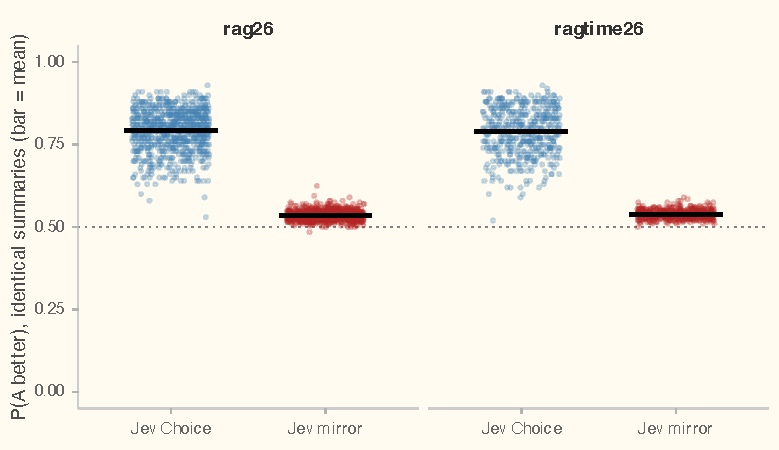
\includegraphics[width=0.5\linewidth]{figures_ggplot/f03_identical_summaries} 

}

\caption{Jev Choice questions exhibit clear order bias in the Pairwise Jev Judge. Using a mirrored version of the choies with order inverted removes most of that bias.}\label{fig:unnamed-chunk-1}
\end{figure}

\subsection{3.2 Pairwise Jev vs BOD Jev + BOD+HR
Jev}\label{pairwise-jev-vs-bod-jev-bodhr-jev}

\begin{figure}

{\centering 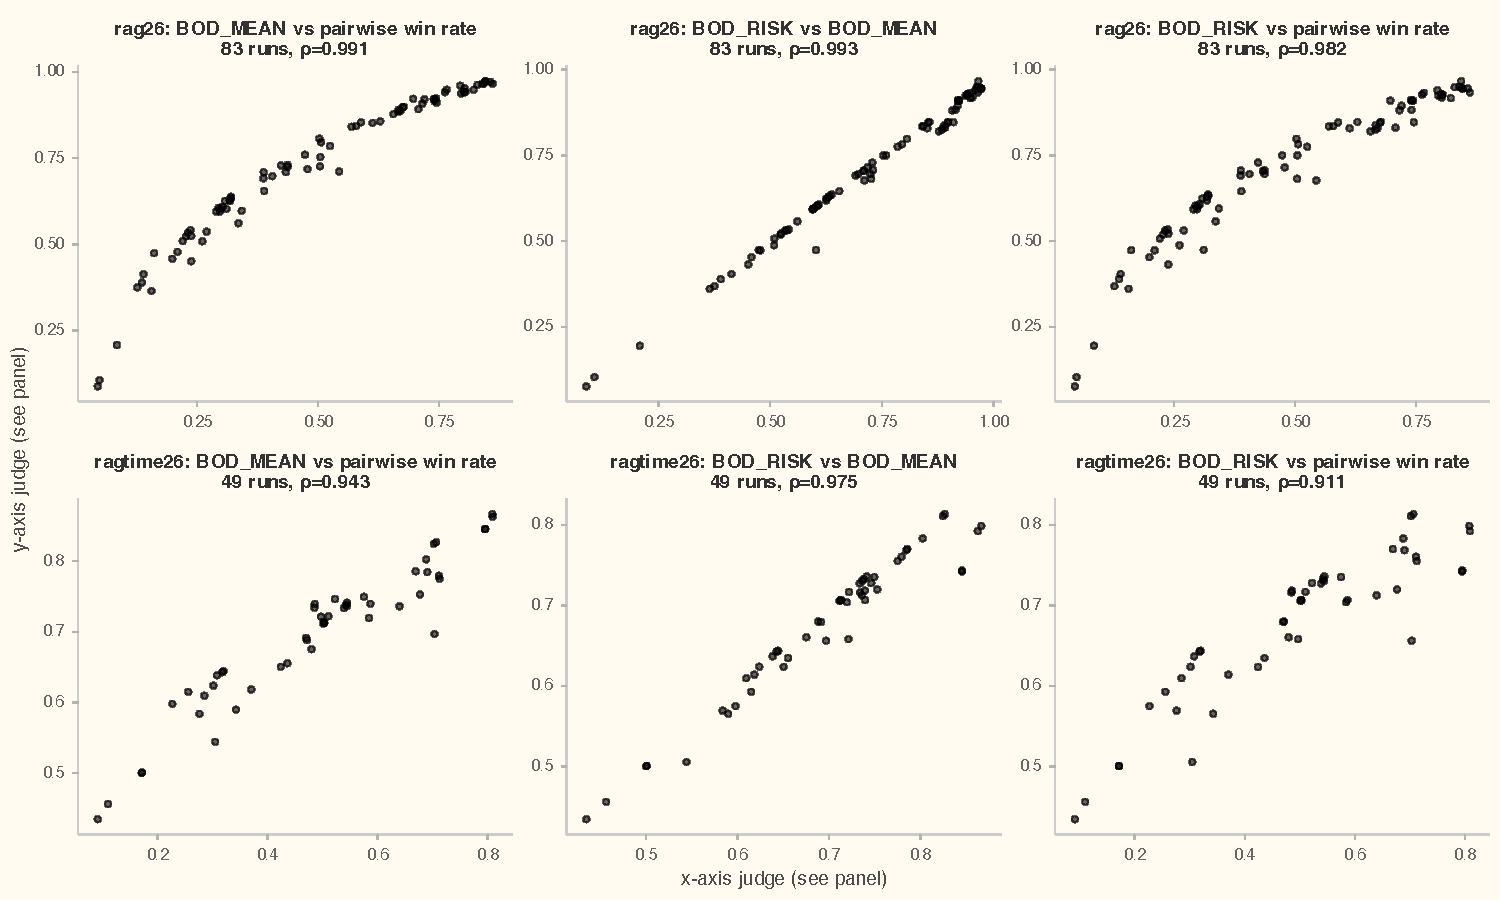
\includegraphics[width=0.5\linewidth]{figures_ggplot/f11_full_leaderboards} 

}

\caption{Comparison of leaderboards created with different Jev Judges. Hallucination Risk (Grounded) makes very little change compared to Bag of Decisions (BOD)}\label{fig:unnamed-chunk-2}
\end{figure}

\subsection{3.2 Judge Jev datum}\label{judge-jev-datum}

There is strong answer correlation across differen question framing
within the same prompt. There are distinc confidence distributions
associtate with SCORE and CHOICE answers.

\section{4. Conclusions}\label{conclusions}

After conference.

\section{5. Appendix}\label{appendix}

\subsection{5.1 OpenRouter Prompts}\label{openrouter-prompts}

\subsubsection{5.1.1 Pairwise Jev}\label{pairwise-jev-1}

\begin{verbatim}
prompt = '
{
  "model": "typesafe/jev-1.13",
  "state": {
    "query": "fall leaf color change chlorophyll",
    "problem_statement": "My 5-year-old keeps noticing that leaves turn red, orange, and yellow in the fall. They want to know why trees change color, whether the leaves are dying, and if the tree will be okay. They also asked why some trees stay green all year and whether cold weather causes the color change.",
    "background": "This is for a child who loves collecting leaves on walks and sorting them by color and shape. They like pressing leaves into notebooks, doing craft projects with them, and comparing different tree leaves side-by-side. They are especially fascinated by bright colors and want explanations that connect to what they can directly see outdoors.",
    "summary_a": "Leaves change color in fall because of a green pigment called chlorophyll. When days get shorter and cooler, trees stop making chlorophyll. Without the green, other colors like yellow and orange can show through. Red colors come from sugars trapped in the leaves. The tree will be fine - it drops leaves to save water for winter.",
    "summary_b": "Trees have green stuff in their leaves called chlorophyll. In fall, the green goes away and you see other colors. Yellow and orange were hiding under the green all along. Some trees like pine trees stay green because they have a different kind of leaf."
  },
  "questions": {
    "better_summary": {
      "type": "choice",
      "instructions": "You are a subject matter expert. Two RAG summaries (summary_a and summary_b) were generated for the query. Which summary better satisfies the information need of the query, considering relevance, completeness, and how well its claims are grounded?",
      "criteria": {
        "A": "summary_a better satisfies the information need of the query.",
        "B": "summary_b better satisfies the information need of the query."
      }
    }
  }
}
'

cat(toJSON(fromJSON(prompt), auto_unbox = TRUE, pretty = TRUE))
\end{verbatim}

\subsubsection{5.1.2 Bag of Decisions Jev}\label{bag-of-decisions-jev}

\paragraph{LLM Bag of Decisions
generation}\label{llm-bag-of-decisions-generation}

\paragraph{Jev Bag of Questions
assembly}\label{jev-bag-of-questions-assembly}

\subsubsection{5.1.3 Judge Jev}\label{judge-jev-1}

\section*{References}\label{references}
\addcontentsline{toc}{section}{References}

\protect\phantomsection\label{refs}
\begin{CSLReferences}{1}{1}
\bibitem[\citeproctext]{ref-bradley1952rank}
Bradley, Ralph Allan, and Milton E. Terry. 1952. {``Rank Analysis of
Incomplete Block Designs: I. The Method of Paired Comparisons.''}
\emph{Biometrika} 39 (3/4): 324--45.
\url{https://doi.org/10.2307/2334029}.

\bibitem[\citeproctext]{ref-honnibal2017spacy}
Honnibal, Matthew, and Ines Montani. 2017. \emph{spaCy 2: Natural
Language Understanding with Bloom Embeddings, Convolutional Neural
Networks and Incremental Parsing}. \url{https://spacy.io}.

\bibitem[\citeproctext]{ref-panickssery2024llm}
Panickssery, Arjun, Samuel R. Bowman, and Shi Feng. 2024. {``LLM
Evaluators Recognize and Favor Their Own Generations.''} \emph{Advances
in Neural Information Processing Systems (NeurIPS 2024)}.
\url{https://arxiv.org/abs/2404.13076}.

\bibitem[\citeproctext]{ref-wang2024large}
Wang, Peiyi, Lei Li, Liang Chen, et al. 2024. {``Large Language Models
Are Not Fair Evaluators.''} \emph{Proceedings of the 62nd Annual Meeting
of the Association for Computational Linguistics (ACL 2024)}, 9440--50.
\url{https://arxiv.org/abs/2305.17926}.

\bibitem[\citeproctext]{ref-wang2020minilm}
Wang, Wenhui, Furu Wei, Li Dong, Hangbo Bao, Nan Yang, and Ming Zhou.
2020. {``MiniLM: Deep Self-Attention Distillation for Task-Agnostic
Compression of Pre-Trained Transformers.''} \emph{Advances in Neural
Information Processing Systems 33 (NeurIPS 2020)}.
\url{https://arxiv.org/abs/2002.10957}.

\bibitem[\citeproctext]{ref-zheng2023judging}
Zheng, Lianmin, Wei-Lin Chiang, Ying Sheng, et al. 2023. \emph{Judging
LLM-as-a-Judge with MT-Bench and Chatbot Arena}.
\url{https://arxiv.org/abs/2306.05685}.

\end{CSLReferences}

\end{document}
